\documentclass[border=10pt]{standalone}
\usepackage{pgfplots}
\usepgfplotslibrary{colormaps}
\pgfplotsset{compat=1.18}

\begin{document}
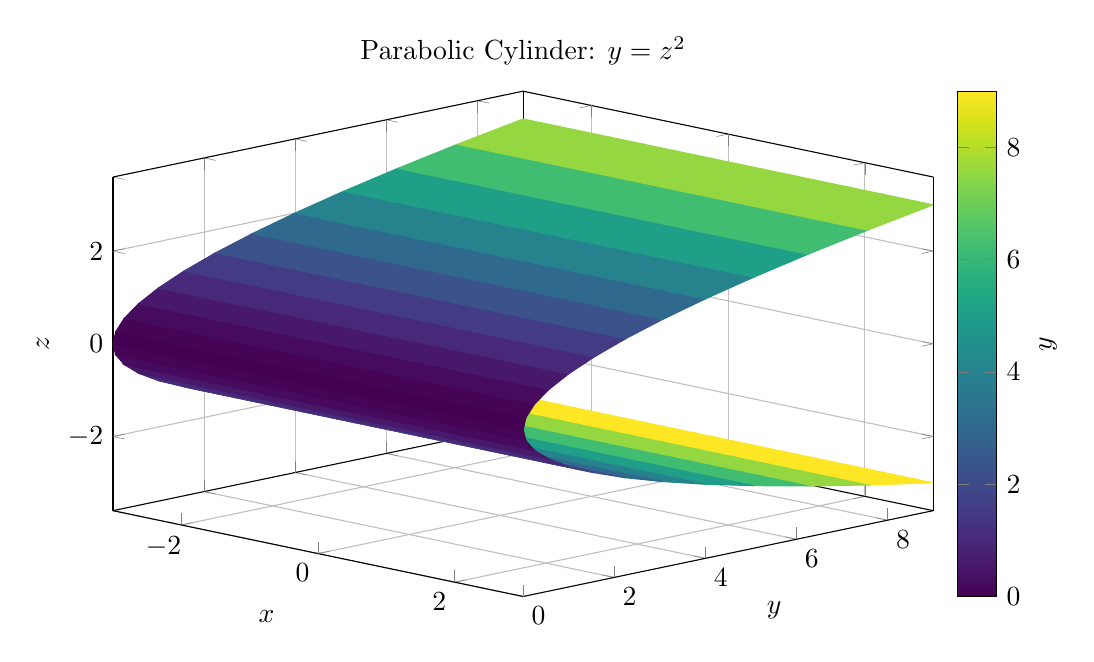
\begin{tikzpicture}
\begin{axis}[
    view={45}{20},
    xlabel=$x$,
    ylabel=$y$,
    zlabel=$z$,
    title={Parabolic Cylinder: $y = z^2$},
    colormap/viridis,
    colorbar,
    colorbar style={
        ylabel={$y$},
    },
    grid=major,
    width=12cm,
    height=8cm,
    samples=25,
    domain=-3:3,
    y domain=-3:3,
    z buffer=auto,
]
\addplot3[surf, shader=flat corner, point meta=y] ({x},{y^2},{y});
\end{axis}
\end{tikzpicture}
\end{document}
